%coding:utf-8

%----------------------------------------
%FOSAPHY, a LaTeX-Code for a summary of optics
%Copyright (C) 2014, Mario Felder, Michael Fallegger

%This program is free software; you can redistribute it and/or
%modify it under the terms of the GNU General Public License
%as published by the Free Software Foundation; either version 2
%of the License, or (at your option) any later version.

%This program is distributed in the hope that it will be useful,
%but WITHOUT ANY WARRANTY; without even the implied warranty of
%MERCHANTABILITY or FITNESS FOR A PARTICULAR PURPOSE.  See the
%GNU General Public License for more details.
%----------------------------------------

\chapter{Quanten Optik}
\section{Konstanten}
\[
\boxed{\begin{aligned}	
		&h = 6.62606872\cdot 10^{-34} J\cdot s \\
		&m_e = 9.1094\cdot 10^{-31}kg \\
		&k_B = 1.380658 \cdot 10^{-23} \frac{J}{K}\\
		&eV = 1.602176565 \cdot 10^{-19}J\\
	\end{aligned}}	\]
\\
\section{Grundformeln}
Umrechnung:
\[
	E_J = E_{eV} \cdot 1.602\cdot 10^{-19}
\]
\\
\section{Photon- das Lichtquantum}
Die maximale kinetische Energie nimmt linear mit der Frequenz des Lichts zu. Es wird kein Photostrom beobachtet für $f<f_0$.\
\[
	E=h\cdot f = \hbar \cdot \omega = \frac{h \cdot c}{\lambda}
\]
\begin{footnotesize}
	$h$:	Planck'sche Konstante = $6.62606872\cdot 10^{-34} J\cdot s$\\
\end{footnotesize}
\begin{center}
	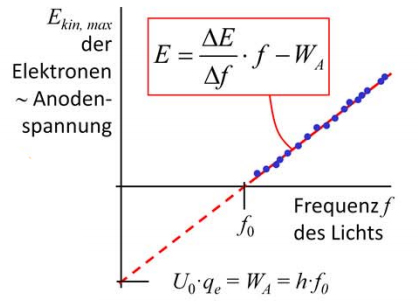
\includegraphics[scale = 0.3]{images/photon_energie.jpg}
\end{center}
\
\\
\section{Impuls des Photons - Compton Streuung}
Obwohl das Photon keine Ruhemasse besitzt, hat es trotzdem einen Impuls. Die Relativitätstheorie liefert für das Photon mit Wellenlänge $\lambda$ den Impuls $p$:\

\[
	p=\frac{E}{c}=\frac{h\cdot f}{c}= \frac{h}{\lambda} \\ \text{pro Photon} \\ \\
\]
Energie- und Impulserhaltung liefern:
\[
	\Delta\lambda = \lambda^` -\lambda=\frac{h}{m_e\cdot c}\cdot \left( 1- \cos \phi  \right) = \lambda_c \cdot \left( 1- \cos \phi   \right) )
\]
Anzahl Photonen pro Sekunde:
\[
	n=\frac{P}{E}
\]
\begin{center}
	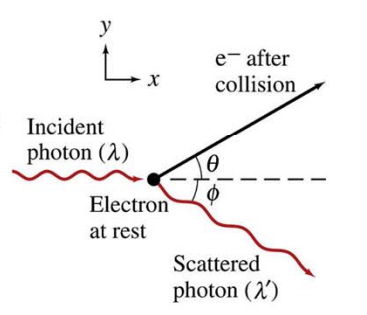
\includegraphics[scale = 0.3]{images/impuls_photon.jpg}
\end{center}
\
\section{Bremsstrahlung}
In einer Röntgenröhre werden Elektronen von einer geheizten  Kathode auf die Anode beschleunigt. Maximale Frequenz (kleinste Wellenlänge) kann ein Bremstrahlungs-Photon erreichen, wenn es die ganze kinetische Energie des Elektrons schluckt.\
\[
	q_e\cdot V_{AC} = h\cdot f_{max} = \frac{h\cdot c}{\lambda_{max}}=\frac{\Delta E}{h\cdot c}
\]
\\
\section{Energieniveaus von Wasserstoff}
Balmer-Formel:
\[
	\frac{1}{\lambda}=R_y\cdot \left( \frac{1}{2^2} - \frac{1}{n^2}\right) 
\]
\begin{footnotesize}
	$R_y$=	$1.097\cdot 10^7 m^{-1}$\\
	$n$=	$3,4,5,...$ \\
\end{footnotesize}
\[
	E_n= -\frac{h\cdot c \cdot R_y}{n^2}
\]
\begin{footnotesize}
	$R_y$=	$1.097\cdot 10^7 m^{-1}$\\
	$n$=	$1,2,3,...$ \\
\end{footnotesize}
\begin{center}
	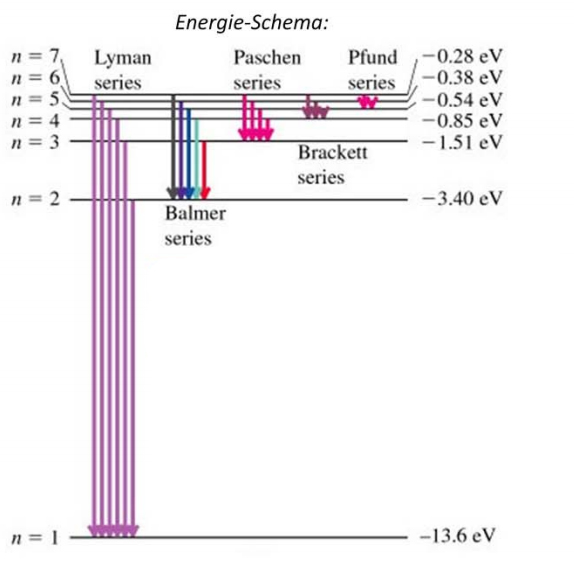
\includegraphics[scale = 0.25]{images/en_H.jpg}
\end{center}
\
\subsection{Bohr's Herleitung der Balmerformel}
Wasserstoff:
\[
	E_n= - \frac{1}{\varepsilon_0^2}\cdot\frac{m_e\cdot q_e^4}{8n^2\cdot h^2}
\]
Helium+:
\[
	E_n= - 
	\frac{1}{\varepsilon_0^2}\cdot\frac{m_e\cdot q_e^4}{2n^2\cdot h^2}
\]
\begin{center}
	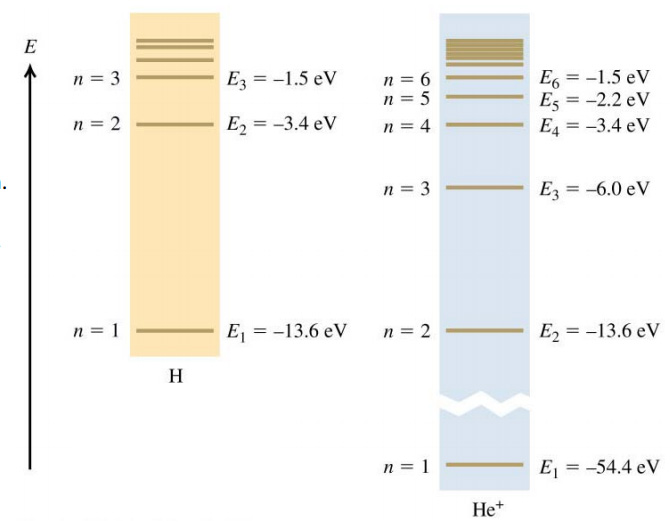
\includegraphics[scale = 0.25]{images/bhor_herleitung.jpg}
\end{center}
\
\\
\section{Energieschema}
\begin{center}
	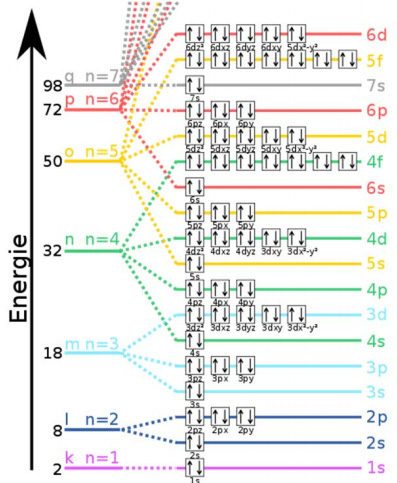
\includegraphics[scale = 0.3]{images/energieschema.jpg}
\end{center}
\
\\
\section{Spektrum des Natriumatoms}
\begin{center}
	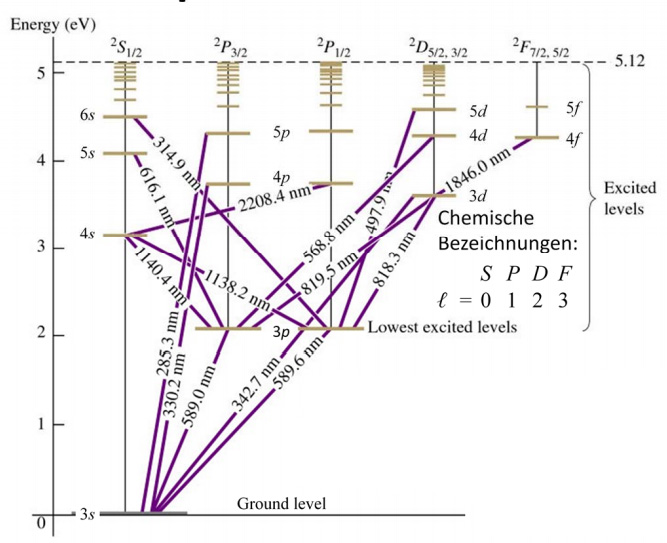
\includegraphics[scale = 0.3]{images/spektrum_na.jpg}
\end{center}
\
\\
\section{Niveaubesetzung und Besetzungsinversion}
Die Maxwell-Boltzmann-Verteilung der Geschwindigkeiten in einem Gas bei der Temperatur $T$ lautet:\
 $f(v,T)=C_1(T)\cdot v^2 e^{-\left( \frac{m_{kül} \ cdot v^2}{2k_B\cdot T} \right) }$\
 oder als Funktion der Energie: $f(E;T)=C_2(T)E\cdot e~{ \frac{E}{k_B\cdot T}}$.\
 \\
 Verhältnis der beiden Besetzungswahrscheinlichkeiten:
 \[
 	\frac{F(E_f,T)}{F(E_i,T)}=\frac{E_f}{E_i}\cdot e^{-\left( \frac{E_f-E_i}{k_B\cdot T}\right) }
 	\approx	
 	e^{-\left( \frac{E_{Gap}}{k_B\cdot T}\right) }
 \]
 \[
 	\frac{f_2}{f_1}=e^{-\left( \frac{1}{k_B\cdot T}  \right) }\left(  E_2-E_1 \right) 
 \]
 \begin{footnotesize}
 	$f$=	$e^{- \frac{E_1}{k_B \cdot T}}$\\
 \end{footnotesize}
 \
 \\
 \section{Quantenverschrkänkung = Superposition}
 $Hg_2$ Molekül:\\
 Wir sind gewohnt Teilsysteme als völlig unabhängig voneinander zu betrachten. Verschränkung bedeutet nun, dass die beiden Atome durch eine gemeinsame Wellenfunktion beschrieben werden. Es handelt sich bei der instanten Spinausrichtung des zweiten Atoms nicht um eine Nachrichtenübertragung im klassischen Sinn. Bei der Messung des ersten Atoms, wird die Ausrichtung des zweiten Atoms festgelegt.\
 \\
 \section{Polarisation und Photonen}
 Die Durchgangswahrscheinlichkeit $p$ der Photonen ist ene Funktion des Winkels $\theta$ (Gesetz von Malus):\
 \[
 	p(\theta)= \cos^2(\theta)
 \]
 \begin{center}
 	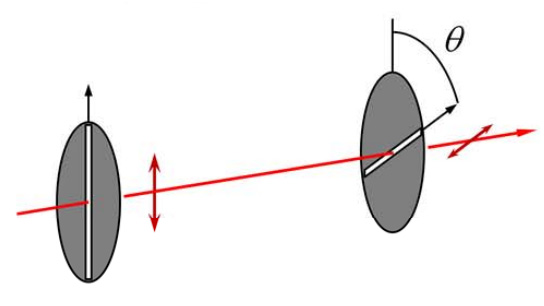
\includegraphics[scale = 0.3]{images/polarisation_photon.jpg}
 \end{center}
 Die Wahrscheinlichkeit, dass das $+z$ polarisierte Teilchen den zweiten Polarisator als $+s$ polarisiertes Teilchen passiert, beträgt:
 \[
 	p(\theta)= \cos^2(\frac{\theta}{2})
 \]
 \\
 \section{Verschränkung mit Photonen}
 Eine Quelle produziere verschränkte Photonenpaare. Die verschränkten Photonen fliegen in entgegengesetzte Richtungen und passieren Polfilter.\
 Die Wahrscheinlichkeit, dass beide Photonen die Filter passieren, ist:
 \[
 	p(\alpha,\beta)= \frac{1}{2} \cdot\cos^2(\alpha-\beta)
 \]
 \begin{center}
 	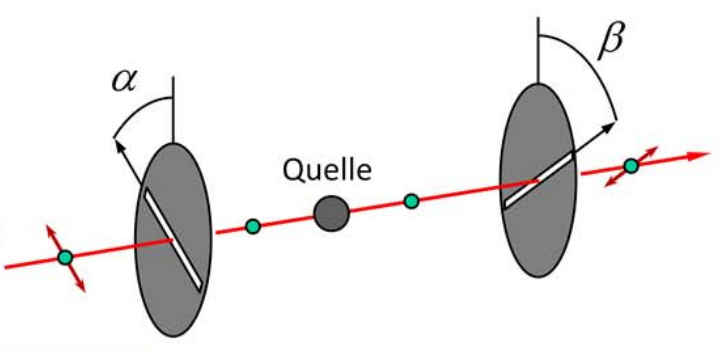
\includegraphics[scale = 0.2]{images/verschraenkung_photon.jpg}
 \end{center}